\section{Observations and Calculations}
	\subsection{Recording the scattering rate\\as function of the angle}

		Our experimentally observed data for measuring the counts and hence the decay rate for different angles is shown in \hyperref[tab:1]{Table 1}. The graph for the same is shown in \hyperref[graph:1]{Figure 4}.

		\begin{table}[h]
	\centering
	\begin{tabular}{|c|c|c|c|}
	\hline
	\textbf{\begin{tabular}[c]{@{}c@{}}Angle\\ $(\theta)$\end{tabular}} & \textbf{Time (s)} & \textbf{Counts} & \textbf{\begin{tabular}[c]{@{}c@{}}Counts per\\ second $N(\theta)$\end{tabular}} \\ \hline
	\multirow{5}{*}{25} & \multirow{5}{*}{600} & 133 & \multirow{5}{*}{0.225} \\ \cline{3-3}
	 &  & 140 &  \\ \cline{3-3}
	 &  & 127 &  \\ \cline{3-3}
	 &  & 137 &  \\ \cline{3-3}
	 &  & 138 &  \\ \hline
	\multirow{5}{*}{20} & \multirow{5}{*}{200} & 164 & \multirow{5}{*}{0.940} \\ \cline{3-3}
	 &  & 198 &  \\ \cline{3-3}
	 &  & 186 &  \\ \cline{3-3}
	 &  & 195 &  \\ \cline{3-3}
	 &  & 197 &  \\ \hline
	\multirow{5}{*}{15} & \multirow{5}{*}{100} & 311 & \multirow{5}{*}{2.929} \\ \cline{3-3}
	 &  & 276 &  \\ \cline{3-3}
	 &  & 277 &  \\ \cline{3-3}
	 &  & 311 &  \\ \cline{3-3}
	 &  & 290 &  \\ \hline
	\multirow{5}{*}{10} & \multirow{5}{*}{100} & 1726 & \multirow{5}{*}{17.626} \\ \cline{3-3}
	 &  & 1811 &  \\ \cline{3-3}
	 &  & 1713 &  \\ \cline{3-3}
	 &  & 1754 &  \\ \cline{3-3}
	 &  & 1809 &  \\ \hline
	\multirow{5}{*}{5} & \multirow{5}{*}{100} & 2931 & \multirow{5}{*}{29.286} \\ \cline{3-3}
	 &  & 2938 &  \\ \cline{3-3}
	 &  & 2912 &  \\ \cline{3-3}
	 &  & 2931 &  \\ \cline{3-3}
	 &  & 2931 &  \\ \hline
	\multirow{5}{*}{-5} & \multirow{5}{*}{100} & 2934 & \multirow{5}{*}{29.343} \\ \cline{3-3}
	 &  & 2933 &  \\ \cline{3-3}
	 &  & 2935 &  \\ \cline{3-3}
	 &  & 2935 &  \\ \cline{3-3}
	 &  & 2935 &  \\ \hline
	\multirow{5}{*}{-10} & \multirow{5}{*}{100} & 1751 & \multirow{5}{*}{17.824} \\ \cline{3-3}
	 &  & 1778 &  \\ \cline{3-3}
	 &  & 1831 &  \\ \cline{3-3}
	 &  & 1787 &  \\ \cline{3-3}
	 &  & 1766 &  \\ \hline
	\multirow{5}{*}{-15} & \multirow{5}{*}{100} & 291 & \multirow{5}{*}{2.940} \\ \cline{3-3}
	 &  & 294 &  \\ \cline{3-3}
	 &  & 289 &  \\ \cline{3-3}
	 &  & 290 &  \\ \cline{3-3}
	 &  & 306 &  \\ \hline
	\multirow{5}{*}{-20} & \multirow{5}{*}{200} & 210 & \multirow{5}{*}{1.009} \\ \cline{3-3}
	 &  & 194 &  \\ \cline{3-3}
	 &  & 211 &  \\ \cline{3-3}
	 &  & 201 &  \\ \cline{3-3}
	 &  & 194 &  \\ \hline
	\multirow{5}{*}{-25} & \multirow{5}{*}{600} & 133 & \multirow{5}{*}{0.225} \\ \cline{3-3}
	 &  & 140 &  \\ \cline{3-3}
	 &  & 127 &  \\ \cline{3-3}
	 &  & 135 &  \\ \cline{3-3}
	 &  & 141 &  \\ \hline
	\end{tabular}
	\caption{Table for $N(\theta)$ for 5mm thick Gold foil}
	\label{tab:1}
\end{table}
		\begin{figure}[h]
			\centering
			\label{graph:1}
			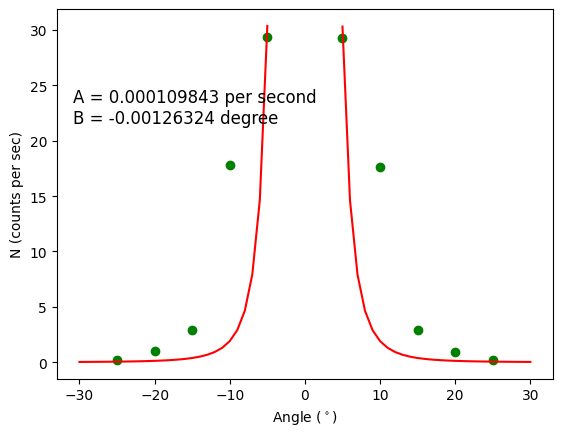
\includegraphics[width=0.8\columnwidth]{images/graph1.png}
			\caption{N vs $\theta$ graph for \hyperref[tab:1]{Table 1}}
		\end{figure}

		In \hyperref[graph:1]{Figure 4} we have fitted the curve with the function:
		$$y = \frac{A}{\sin^4\frac{x-B}{2}}$$

		where $A$ and $B$ are the constants to be determined, $x$ is the angle $(\theta)$ and $y$ is the counts per second.

		From \hyperref[graph:1]{the graph} we got the values of the constants as:

		$$A = 0.000109843 = 1.098\times10^{-4}\text{ per second}$$
		$$B = -0.00126324 = 1.263\times10^{-3}\text{ degree}$$
	
	\subsection{Determining the atomic number of Al}

		Our experimentally observed data for measuring the counts and hence the decay rate for different materials keeping all other conditions constant is shown in \hyperref[tab:2]{Table 2}.

		\begin{table}[H]
    \centering
    \begin{tabular}{|c|c|c|c|}
        \hline
        $V_{DC}$ & $V_{DUT}$ & $V_{OUT}$ & $C_{DUT}$   \\ \hline
        0        & 0.074     & 0.459     & 127.837 \\
        0.1      & 0.109     & 0.451     &  85.276 \\
        0.2      & 0.232     & 0.447     &  39.709 \\
        0.3      & 0.299     & 0.438     &  30.191 \\
        0.4      & 0.389     & 0.432     &  22.888 \\
        0.5      & 0.463     & 0.432     &  19.230 \\
        0.6      & 0.564     & 0.426     &  15.567 \\
        0.7      & 0.662     & 0.420     &  13.075 \\
        0.8      & 0.760     & 0.435     &  11.796 \\
        0.9      & 0.846     & 0.430     &  10.475 \\
        1        & 0.941     & 0.426     &   9.330 \\
        1.1      & 1.058     & 0.427     &   8.318 \\
        1.2      & 1.174     & 0.422     &   7.408 \\
        1.3      & 1.267     & 0.418     &   6.799 \\
        1.4      & 1.357     & 0.416     &   6.318 \\
        1.5      & 1.464     & 0.412     &   5.800 \\
        1.6      & 1.559     & 0.409     &   5.406 \\ \hline
    \end{tabular}
    \caption{Data for light condition}
    \label{tab:2}
\end{table}

		Now, we know that:
		\begin{itemize}
			\item $Z_{Au}$ = 79
			\item We used equal thickness foils. So, $d_{Au}$ = $d_{Al}$.
			\item $N_{Au} = 0.48cps$ 
			\item $N_{Al} = 0.01333cps$.
		\end{itemize}

		from \hyperref[eq:2]{Equation 2} we get the value of $Z_{Al}$ as:

		$$Z_{Al} = 79\sqrt{\frac{0.01333}{0.48}}$$

		$$\fbox{Z = 13.167}$$
